\RequirePackage{fix-cm}
\RequirePackage[hyphens]{url}
\RequirePackage[final]{graphicx} % need to show figures in draft mode
\documentclass[rmp,nofootinbib,superscriptaddress,12pt,tightenlines,notitlepage]{revtex4-1}

\setlength\topmargin{0pt}
\addtolength\topmargin{-\headheight}
\addtolength\topmargin{-\headsep}
\setlength\oddsidemargin{0pt}
\setlength\textwidth{\paperwidth}
\addtolength\textwidth{-2in}
\setlength\textheight{\paperheight}
\addtolength\textheight{-2in}
\usepackage{layout}

% Change to a sans serif font.
\usepackage{sourcesanspro}
\renewcommand*\familydefault{\sfdefault} %% Only if the base font of the document is to be sans serif
\usepackage[T1]{fontenc}
%\usepackage[font=sf,justification=justified]{caption}
\usepackage[font=sf]{floatrow}

% Rework captions to use sans serif font.
\makeatletter
\renewcommand\@make@capt@title[2]{%
 \@ifx@empty\float@link{\@firstofone}{\expandafter\href\expandafter{\float@link}}%
  {\textbf{#1}}\sf\@caption@fignum@sep#2\quad
}%
\makeatother

%\linespread{0.956}
\usepackage{listings} % For code examples
\usepackage[usenames,dvipsnames,svgnames,table]{xcolor}
\usepackage{amsmath}
\usepackage{amssymb}
\usepackage{graphicx}
\usepackage{dcolumn}
\usepackage{boxedminipage}
\usepackage[colorlinks=true,citecolor=blue,linkcolor=blue]{hyperref}
\usepackage[]{microtype}
\usepackage[obeyFinal]{todonotes}
\usepackage{import}
\usepackage{setspace, siunitx, amsmath,amsfonts, adjustbox,booktabs, cleveref}
%\usepackage{caption}
\usepackage{subcaption}
\usepackage{titlesec}
\usepackage{enumitem}
\usepackage[margin=1.0in]{geometry}
\usepackage{etoolbox}
\patchcmd{\section}
  {\centering}
  {\raggedright}
  {}
  {}
\patchcmd{\subsection}
  {\centering}
  {\raggedright}
  {}
  {}
\usepackage{wrapfig}
\graphicspath{{/home/bmanubay/Bryces-prelim-exam/report/images/}}

\usepackage{parskip}
\setlength{\parskip}{4pt} % 1ex plus 0.5ex minus 0.2ex}
\setlength{\parindent}{0pt}

\setcitestyle{super}
\setcounter{secnumdepth}{5}

% Units
\DeclareSIUnit\Molar{\textsc{m}}


% Comments
\newcounter{comment}
\newcommand{\comment}[2][]{%
% initials of the author (optional) + note in the margin
\refstepcounter{comment}%
{%
\setstretch{0.7}% spacing
\todo[inline, color={cyan!45},size=\small]{%
\textbf{\footnotesize [\uppercase{#1}\thecomment]:}~#2}%
}}

% Start supplementary sections

\newcommand{\beginsupplement}{%
        \onecolumngrid
        \setcounter{table}{0}
        \renewcommand{\thetable}{S\arabic{table}}%
        \setcounter{figure}{0}
        \renewcommand{\thefigure}{S\arabic{figure}}%
     }

%\graphicspath{{figures/}}
\floatsetup[table]{capposition=top}

\titlespacing\title{4pt}{12pt plus 4pt minus 2pt}{4pt plus 2pt minus 1pt}
\titlespacing\section{0pt}{12pt plus 4pt minus 2pt}{0pt plus 2pt minus 2pt}
\titlespacing\subsection{0pt}{12pt plus 4pt minus 2pt}{0pt plus 2pt minus 2pt}
\titlespacing\subsubsection{0pt}{12pt plus 4pt minus 2pt}{0pt plus 2pt minus 2pt}

\begin{document}

%%%%%%%%%%%%%%%%%%%%%%%%%%%%%%%%%%%%%%%%%%%%%%%%%%%%%%%%%%%%%%%%%%%%%%%%%%%%%%%%
% DOCUMENT
%%%%%%%%%%%%%%%%%%%%%%%%%%%%%%%%%%%%%%%%%%%%%%%%%%%%%%%%%%%%%%%%%%%%%%%%%%%%%%%%

\title{A method for redesigning molecular mechanics force field parameterization by use of a Bayesian statistical framework\vspace{-2ex}}
\author{Bryce C. Manubay\vspace{-2ex}} 
\email{bryce.manubay@colorado.edu}
\affiliation{University of Colorado - Department of Chemical and Biological Engineering\vspace{-2ex}}
% Date
\date{\today\vspace{-2ex}}

%%%%%%%%%%%%%%%%%%%%%%%%%%%%%%%%%%%%%%%%%%%%%%%%%%%%%%%%%%%%%%%%%%%%%%%%%%%%%%%%
% ABSTRACT
%%%%%%%%%%%%%%%%%%%%%%%%%%%%%%%%%%%%%%%%%%%%%%%%%%%%%%%%%%%%%%%%%%%%%%%%%%%%%%%%
{\Large \textbf{A method for redesigning molecular dynamics force field parameterization by use of a Bayesian statistical framework}}

\hspace{0.5 in} Bryce C. Manubay

\hspace{0.5 in} \textit{University of Colorado - Department of Chemical and Biological Engineering}

\hspace{0.5 in} (Dated: \today) 


\section{Objectives}
Molecula  dynamics (MD) simulation is fast becoming a more useful tool in many scientific studies. 
However, some limitations remain in the ability of MD force fields to accurately and transferably 
describe molecular environments. Many popular and currently used force fields were parameterized 
with fixed functional forms which, often, have poor physical motivation. The chemical intuition of 
experts is also often required to manually correct parameters, leading to a more suitable product. 
Additionally, the creation of a transferable method to update existing force fields based on new 
experimental data is limited due to lack of understanding and lack of consistency in how the original 
parameterizations were done.

A possible solution to these problems is by recasting the force field parameterization process as a 
bayesian inference problem. The objective of this paper is introduce a framework for using high quality 
experimental data in order to automatically generate families of MD force fields consistent with the data 
used. In this paper I will generally describe the overall parameterization framework and my roles in the project 
thus far. First, collecting and curating large amounts of high quality experimental thermochemical data 
and, currently, investigating use of the Multistate Bennett Acceptance Ratio (MBAR) as a means to improve 
parameterization throughput by reducing computational expense while making updates to the posterior distribution 
of parameter sets consistent with experimental data provided.

\section{Significance}
A broad variety of research from drug discovery to metallurgy has been greatly impacted by the advent and 
improvement of MD simulation tools. Observing physical phenomena such as protein folding dynamics and ligand 
docking at a molecular scale is widely studied using MD tools.\cite{villin,villin2} Drug discovery and deisgn 
of new pharmaceutical leads has also been made more efficient.\cite{drug_discov} The fundamental part in molecular 
simulation for describing the energetic interactions of a system is referred to as a force field. Hence, 
the development of force fields which are readily transferable between dissimilar physical systems and are 
quantitatively accurate is imperative for the use of molecular simulation tools to continue to proliferate.

Transferability of MD force fields, and particularly sets of force field parameters, is an extremely popular 
topic (and current limitation) in the molecular simulation field.\cite{transferability1,transferability2,
transferability3,transferability4} Transferability of force fields encourages use by providing convenience 
for scientists with wide arrays of research interests and by making parameter space less complex through 
generalization by chemical similarity. Inaccurate and poorly parameterized force fields have been shown to 
grossly misrepresent molecular systems.\cite{ffcomp1,ffcomp2,robustness} 

A few notable attempts, such as GAAMP and ForceBalance, have been made in recent years towards the development of more automated and systematic 
force field parameterization methods.\cite{GAAMP,FB1,FB2,FB3} Each made important contributions to automated 
force field parameterization through clever use of objective function optimization, exploiting a variety of 
fitting data and allowing exploration of functional forms. However, none provided the ability for the computer 
to automatically and systematically explore choices of fitting data, optimization algorithm and functional 
forms in order to objectively find families of force fields consistent with fitting data and reward those with 
the least model complexity. The bayesian inference scheme described in this paper will provide a workflow for 
discovering families of force field parameters consistent with experimental data and a variety of functional forms.

Additionally, as I will demonstrate later in my discussion of data mining and curation of the NIST ThermoML database,
the chemical diversity in readily available thermochemical databases is lacking. Not only that, but the distribution of data
amongst commonly measured properties is heavily skewed towards certain properties. Having learned this since beginning the
project, one of the potential uses of the parameterization scheme is to fill in the many gaps in experimental thermochemical 
data. With updated general descriptions of chemical space and property data on chemically similar compounds, this parameterization
process should provide force fields to accurately simulate property data for which no experimental data exists. 

\section{Background and related literature $\left(1.5 pages \pm 0.5 pages\right)$}
Molecular dynamics force fields define how to construct the potential energy functions (and thereby the forces) 
of an atomistic system under study. The potential is constructed such that it is a function of solely the atomic 
coordinates and a set of parameters associated with the force field. Transferable force fields generally have 
three major parts: 
  \begin{itemize}
   \item [1] The \textbf{functional forms} of the potential, i.e. the mathematical equations for the energy equation. A classic example of a non-bonded interaction form is the 12-6 Lennard-Jones (LJ) potential.   
   \item [2] \textbf{Atom types} which describe similar chemical environments such that one can assign different atoms (or series of atoms) identical parameters, thereby shrinking the parameter space and helping to avoid overfitting.
   \item [3] \textbf{Parameters} that are associated with one or many atom types which determine the magnitude of the interactions in the system 
  \end{itemize}
Rolled into functional forms, \textbf{combining rules} are also sometimes considered. \textbf{Combining rules} describe how to combine parameters 
when an interaction contains multiple atom types.

There are severe limitations in current methods for force field parameterization. Until very 
recently, force fields have primarily been made manually, guided by experimental and quantum chemical simulation 
data as well as the intuition of expert computational chemists.\cite{charmm1,charmm2,mm2,mmff,amber} Some functional 
forms used in modern force fields, like the 12-6 LJ potential, have poor physical basis. While the attractive term 
of the LJ potential has physical basis on the true behavior of dispersion forces, the repulsive term loosely 
approximates Pauli repulsion and is used for computational convenience. Despite attempts at improvement, many of 
the functional forms and parameters of popular force fields remain mostly unchanged due to the lack of clear, 
systematic methods for updating them.\cite{unchanged}

Parameterization methods have slowly become more sophisticated over the last decade and a 
half with advances in computational power and to accommodate modeling increasingly more complex systems. Many early 
force fields were parameterized manually for narrow classes of molecules with large redundant parameter spaces.\cite{mm1} Force fields like AMBER 
\textit{parm94} showed intuitive departure by shrinking parameter space with clever atom typing defined by expert 
computational chemists.\cite{parm94} The parameterization of GAFF used a semi-automated genetic algorithm approach 
to select parameters.\cite{amber} Even more sophisticated optimization approaches such as least-squares optimization 
of an objective function have been utilized in the creation of the TIP4P-Ew water model\cite{tip4pew} and in the 
ForceBalance parameterization scheme\cite{FB1,FB2,FB3}. Even with these more sophisticated optimization schemes there 
are still issues in needing for the user to assign weights to different kinds of data (i.e. different properties) when 
they are included in the same objective function. Molecular systems aren't necessarily uniquely defined by a single 
parameter set. There are possibilities of multiple optima in parameter space (i.e. different sets of parameters that 
all are consistent with data used during parameterization) and least-squares optimization does not discriminate the 
global optima from the other possibilities.

Bayesian inference provides a robust statistical framework for force field parameterization. It has been shown that 
bayesian approaches can be applied to a wide variety of data driven sciences. It's been used for balancing data to 
help minimize influence of oversampled populations and generate more robust predictive models\cite{bayes_imbalance} 
to recalibrating initial force estimates in coarse grained MD models to target atomistic MD and experimental data
\cite{bayes_coarse}. Baye's theorem clearly provides a framework for the problem at hand thusly:
\begin{equation} P\left(\theta|D\right) \propto P\left(D|\theta\right) P\left(\theta\right)\end{equation}\\*
In \textbf{Equation (1)}, consider a model $M$ (including functional forms and atom types) with some unknown set of 
parameters which produced data $D$. $\theta$ is a choice of parameters consistent with data $D$. What \textbf{equation 
(1)} states is that the probability of $\theta$ given $D$ (the \textit{posterior}) can be determined from the probability 
of observing $D$ given $\theta$ (the \textit{likelihood function}) and the probability of $\theta$ (the \textit{prior}). The 
\textit{prior} is imposed by physical constraint or by the previous round of inference. Note that in 
iterative bayesian inference, the posterior of the previous round becomes the prior in the new iteration. This bayesian 
inference produces not just a single parameter set, but an entire posterior distribution of parameters given data. This is advantageous 
given that many different parameter sets can be consistent with the data used and the distribution of these consistent 
sets of parameters can inform what new data could help narrow the distribution and improve the parameter estimates. 
 \begin{figure}[h!]
  \centering
  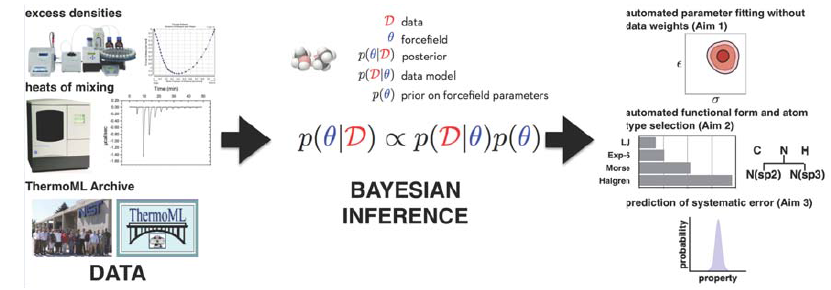
\includegraphics[width=1.0\textwidth]{Bayesian_inference_workflow}
  \caption{A schematic overview of the bayesian inference workflow where force field parameters are inferred given experimental data and a model}
 \end{figure}

The remaining \textbf{Methods} and \textbf{Progress} sections will be split it into two parts each. The first will address the 
problem of gathering, categorizing and curating large amounts of experimental thermochemical data for use as evidence in the 
bayesian inference scheme. The second part will discuss how to address decreasing the computational expense of the simulations
required for the parameterization process using MBAR to estimate simulated properties at new parameter states.  

\subsection{Methods $\left(1.5 pages \pm 0.5 pages\right)$}
\subsubsection{Data mining and curation of thermochemical data in ThermoML}
The experimental thermochemical data to be used for the parameterization process was collected from the NIST ThermoML database managed by the 
Thermodynamics Research Center at the  NIST Boulder campus. In order to explore the composition of the data in ThermoML I used the \textit{ThermoPyL}
Python tool developed by the Chodera lab at the Memorial Sloan Kettering Cancer Center.\cite{thermopyl} The \textit{ThermoPyL} tool parses the
standard ThermoML XML format into a Pandas dataframe format. Further filters can be applied to the dataframes to filter by chemical composition, 
properties of thermodynamic state such as temperature or pressure, as well as thermochemical properties available.

The first planned novel use of the bayesian parameterization procedure is to parameterize a general force field for simulating small organic liquids
and their mixtures. Other than being a concrete test case with readily available experimental data, this choice is motivated by shortcomings of current
force fields to accurately describe organic liquid mixtures (and particularly excess properties).\cite{mix} Given this apparent problem the properties
selected to be used in the pool of potential evidence were chosen for the purpose of more fully constraining parameter space with the goal of being 
able to accurately simulate properties of organic liquid mixtures. The properties chosen from neat liquid data were mass density, isobaric heat capacity, 
speed of sound and static dielectric constant. The properties chosen from the binary mixture data were mass density, speed of sound, static dielectric constant, excess molar volume, excess molar isobaric heat capacity, excess molar enthalpy and infinite dilution activity coefficients. To consider how these properties
might affect the constraint of parameter space one must simply think intuitively about the physics. First, consider mass density. Ultimately, the value of mass 
density for a bulk liquid is determined by the volume of the system and therefore the space between molecules. Therefore, the most important parameters for 
this simulated quantity would be for those describing the non-bonded interactions between molecules. As a counterexample consider the static dielectric constant, 
which is a function of the system dipole moment or more generally electrostatics. Clearly, accurately simulating this property would require constraints placed 
on some electrostatic potential and potentially parameters controlling harmonic bond potential.

\begin{wrapfigure}{r}{0.5\textwidth}
 \centering
 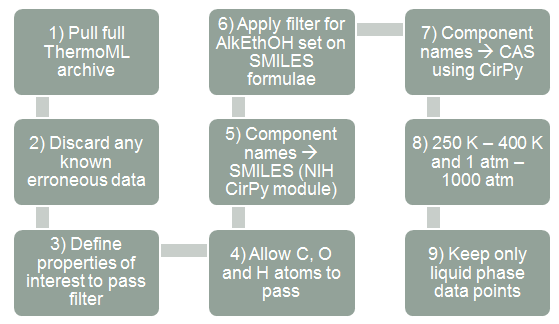
\includegraphics[width=0.9\textwidth]{ThermoML_workflow}
 \caption{A simplified diagram of the filtering algorithm used to find experimental data for use as evidence}
\end{wrapfigure}
A flow diagram representing the filtering process is shown in \textbf{figure 2}. The process is started by organizing a locally stored version of the 
ThermoML database into a Pandas dataframe. First, a filter is applied to discard journal articles with known erroneous data. Next, we filter all data if it doesn't 
fall within our previous properties of interest list. Filters for chemical composition and bond order are next applied, specifically it was decided that for initial 
testing to only look at organics containing C, O and/or H atoms with single or aromatic bonding. Additionally, the molecules had another filter that they must appear
in a diverse list of alkanes, ethers and alcohols (coined AlkEthOH) that was constructed by Chris Bayly of OpenEye Software. AlkEthOH represents a limited test set 
to validate the machinery for parameterization. Finally, only data with temperatures  
250 - 400 K and pressures 1 - 1000 atm are kept in the liquid phase are kept. The data is then saved in an easily machine-readable format such as JSON or PKL. Additionally, potential data 
for use as evidence was sent to the the TRC for validation of quality. The likelihood function described earlier will be a function of uncertainties associated
with the evidence, thus accurate estimates are imperative. The TRC group led by Ken Kroenlein have internally kept estimates for uncertainties of all data points
in ThermoML. Thus, their screening involves checking their uncertainty estimates against what authors published and noting any outliers. 

\subsubsection{Exploring use of multistate reweighting to reduce computational expense}
During each update of iterative bayesian inference, evaluation of the likelihood function will require new simulated evidence given a perturbed parameter set. However, with phase space overlap, new evidence at adjacent states can be estimated using multistate reweighting tools such as MBAR. \cite{MBAR} Given MBAR has a much higher computational efficiency that fully simulating a new state, this could greatly accelerate full construction of a posterior distribution of parameters. \textit{Equation 3} shown below is the formulation that allows for reduced free energies to be found at other states using a simulated state as reference, i.e. it allows for the solution of free energy differences.


Where $u$ is a reduced potential energy, $x$ is a configuration, $K$ is the number of states and $N$ is the number of configurations from the state. These free energy calculations also allow for estimating expectation values of certain obserables at the other thermodynamic states for which relative free energies were calculated. This is done by calculating relative weights of the sampled state to the unsampled states using the formulations shown below in \textbf{equations 4,5 and 6}.


Where $A(x_n)$ is some mechanical observable, $W_{na}$ is a weight and $\hat{A}$ is the estimated expectation of $A(x)$. 

The goal of this exercise is to see how large of parameter perturbations can be made and still make accurate estimates of some observable at that new perturbed state. For this testing phase we've chosen a toy problem of using single molecule simulation observables, such as bond lengths and angles, as the evidence for verifying the validity of the bayesian inference process in the least computationally expensive manner. For testing the safe extent of parameter perturbation I have devised a simple scheme for comparison of reweighted observable estimates to a true sampled value. 




\begin{itemize}
 \item Data Mining and curation from ThermoML
  \begin{itemize}
   \item ThermoPyL
   \item Filtering algorithm(s)
   \item Some stats on total database
   \item Some of the different tests/sets we searched for to check size of chemical environment
   \item AlkEthOH
  \end{itemize}
 \item Reweighting workflow to determine length of jumps allowable in parameter space
  \begin{itemize}
   \item Purpose of reweighting workflow
   \item Brief overview of MBAR maybe
   \item Criteria for safe jump and motivation behind that
   \item Simulations ran
  \end{itemize}
\end{itemize}  
All the stats from the data mining shit

Potential figure from results of jump tests



\subsection{Progress $\left(1.5 pages \pm 0.5 pages\right)$}

\subsection{Research plan $\left(0.5 pages\right)$}

\bibliographystyle{IEEEtran}
\bibliography{report_outline}

\end{document}
